\clearpage
\section{Транзакции}

\subsection{Постановка задачи}
Реализовать сценарий взаимодействия двух пользователей с базой данных с
помощью транзакций и проверить наличие аномалии при выбранном уровне изоляции.
В качестве уровня изоляции выбран \texttt{READ COMMITTED}, а в качестве
проверяемой аномалии — неповторяемое чтение.

\subsection{Выполнение задания}
Для проверки используются созданные ранее учётные записи А и Б с правами,
описанными в предыдущем разделе. Пользователь А может читать статистику
автомобилей, а пользователь Б — добавлять тревожные события. Созданный ранее
триггер увеличивает счётчик тревог после вставки события. Эксперимент проводится
на существующих данных, новая таблица не создаётся.

Сначала в отдельном сеансе пользователя А запускается транзакция и считывается
текущее значение счётчика автомобиля с идентификатором 1. Транзакцию нужно
оставить открытой, не выполняя \texttt{COMMIT}.

\begin{lstlisting}[style=sqlstyle, caption={Пользователь А: начало транзакции и первое чтение}, label={lst:transaction-a-first}]
BEGIN ISOLATION LEVEL READ COMMITTED;

SELECT car_id, alert_count
FROM car_stats
WHERE car_id = 1;
-- Результат проверки: alert_count = 5
\end{lstlisting}

Пока транзакция А остаётся открытой, в отдельном сеансе пользователя Б
добавляется тревожное событие. Команда возвращает идентификатор созданной
записи; его нужно сохранить, чтобы удалить именно тестовое событие после
проверки. После \texttt{COMMIT} изменение счётчика становится доступно другим
транзакциям.

\begin{lstlisting}[style=sqlstyle, caption={Пользователь Б: добавление тревожного события}, label={lst:transaction-b-insert}]
BEGIN ISOLATION LEVEL READ COMMITTED;

INSERT INTO alert_event (
    car_id, alert_event_type_id, status_id, description
)
VALUES (
    1, 1, 1, 'ЛР: проверка READ COMMITTED'
)
RETURNING alert_event_id;

COMMIT;
\end{lstlisting}

После завершения транзакции Б пользователь А повторяет тот же запрос в своей
всё ещё открытой транзакции. Затем транзакция А завершается.

\begin{lstlisting}[style=sqlstyle, caption={Пользователь А: повторное чтение и завершение}, label={lst:transaction-a-second}]
SELECT car_id, alert_count
FROM car_stats
WHERE car_id = 1;
-- Результат проверки: alert_count = 6

COMMIT;
\end{lstlisting}

\subsection{Результаты выполнения}
Последовательность действий пользователей и полученные результаты приведены
в таблице~\ref{tab:transaction-results}.

\begin{table}[htbp]
\centering
\small
\setlength{\tabcolsep}{5pt}
\renewcommand{\arraystretch}{1.2}
\begin{tabularx}{\linewidth}{|c|X|X|}
\hline
\textbf{№} & \textbf{Пользователь \texttt{user\_a}} & \textbf{Пользователь \texttt{user\_b}} \\
\hline
1 & Начинает транзакцию \texttt{READ COMMITTED} и читает \texttt{alert\_count = 5}. Транзакцию оставляет открытой. & — \\
\hline
2 & Ожидает, не завершая транзакцию. & Добавляет строку в \texttt{alert\_event}. Триггер увеличивает \texttt{alert\_count}; команда возвращает идентификатор события, затем выполняется \texttt{COMMIT}. \\
\hline
3 & Повторно читает ту же строку и получает \texttt{alert\_count = 6}; завершает транзакцию командой \texttt{COMMIT}. & — \\
\hline
4 & — & Удаляет тестовое событие по полученному \texttt{alert\_event\_id}. Триггер уменьшает счётчик до исходного значения. \\
\hline
\end{tabularx}
\caption{Результаты проверки неповторяемого чтения}
\label{tab:transaction-results}
\end{table}

Для наглядного подтверждения результаты сеансов приведены отдельно на рисунках~\ref{fig:transaction-user-a} и~\ref{fig:transaction-user-b}.

\begin{figure}[htbp]
\centering
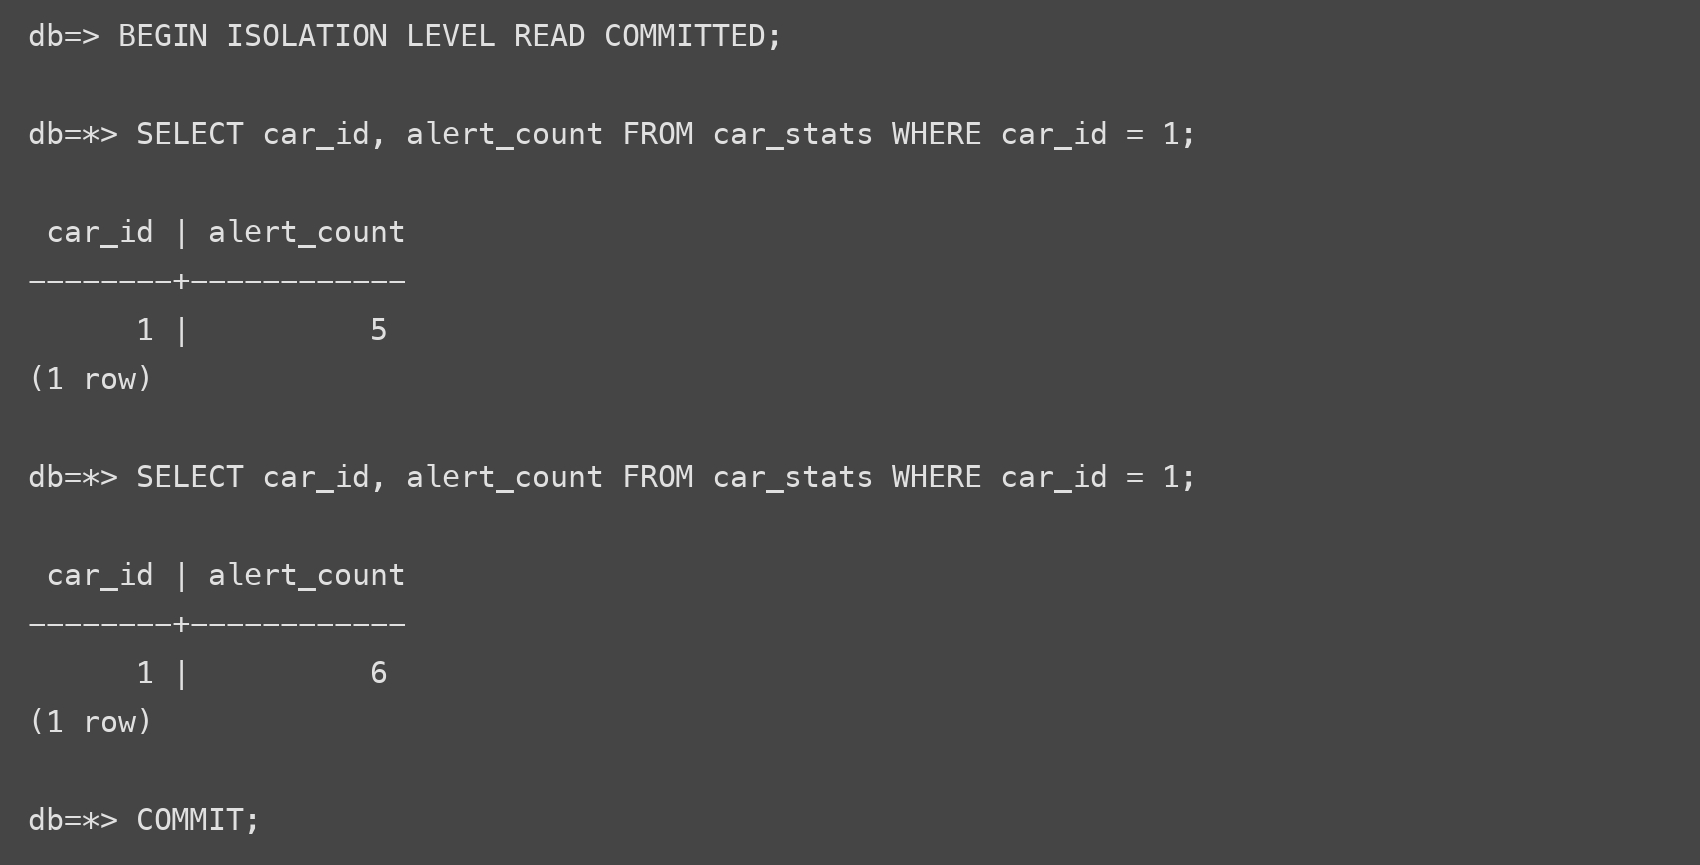
\includegraphics[width=0.92\linewidth]{myPhoto/transaction_user_a.png}
\caption{Сеанс пользователя \texttt{user\_a}: неповторяемое чтение счётчика}
\label{fig:transaction-user-a}
\end{figure}

\begin{figure}[htbp]
\centering
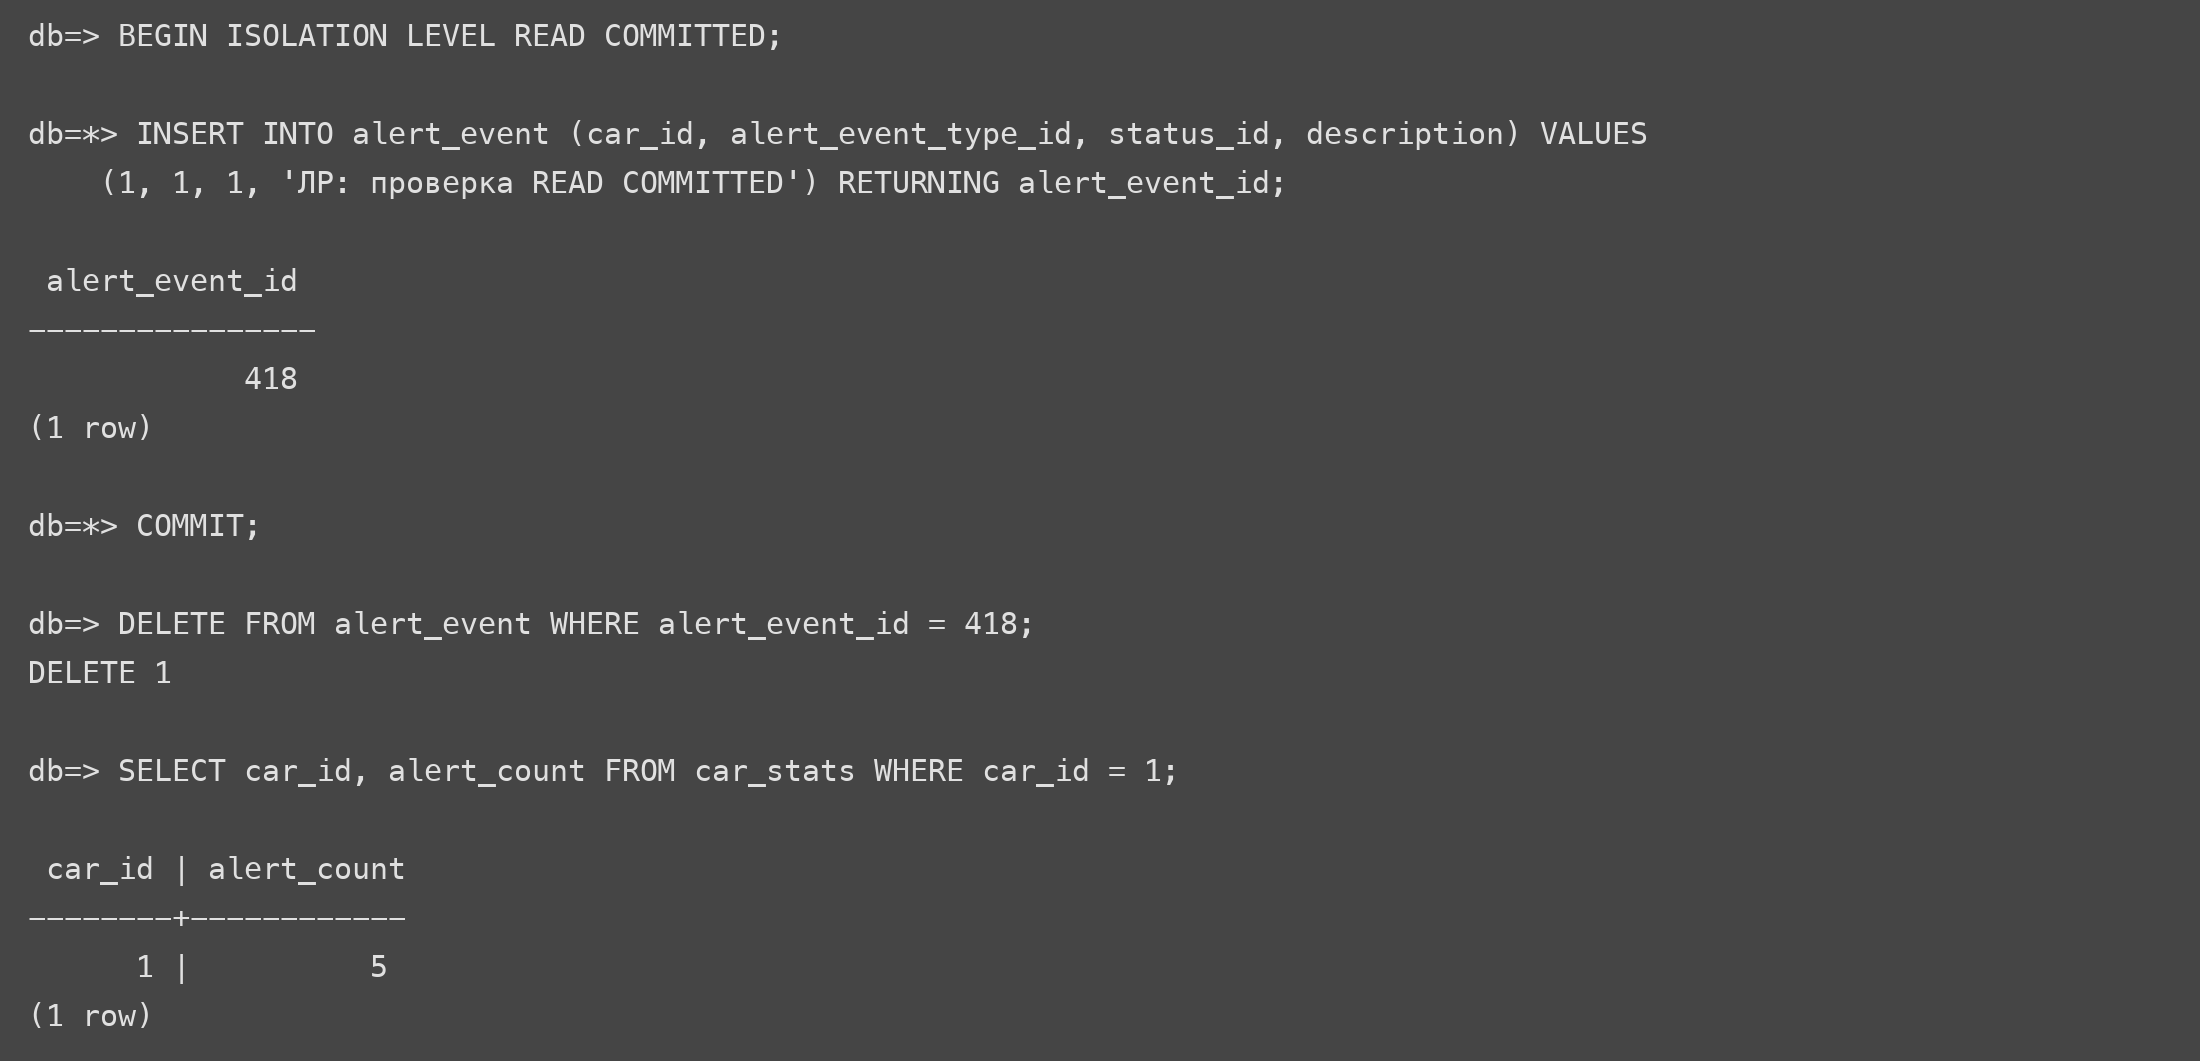
\includegraphics[width=0.92\linewidth]{myPhoto/transaction_user_b.png}
\caption{Сеанс пользователя \texttt{user\_b}: изменение счётчика добавлением тревожного события}
\label{fig:transaction-user-b}
\end{figure}

Для удаления тестовой записи пользователь Б подставляет идентификатор,
полученный в листинге~\ref{lst:transaction-b-insert}:

\begin{lstlisting}[style=sqlstyle, caption={Удаление тестового тревожного события}, label={lst:transaction-cleanup}]
DELETE FROM alert_event
WHERE alert_event_id = 418;
-- При повторном запуске подставить ID из результата INSERT
\end{lstlisting}



\subsection{Вывод}
Сценарий подтвердил наличие неповторяемого чтения. Уровень изоляции —
READ COMMITTED.
Пользователь А в одной транзакции сначала получил значение счётчика 5, а после
фиксации изменения пользователем Б — 6. Это возможно, потому что на уровне
READ COMMITTED каждый оператор получает новый снимок данных. Поэтому два
запроса в одной транзакции могут видеть разные зафиксированные значения.
